
%--------------------------------------------------------------------------
\chapter{INTRODUCTION}

\vspace{3em}
\setlength{\epigraphwidth}{0.86\textwidth}
\setlength{\epigraphrule}{0pt}
\epigraph{
	\textit{Music has become an almost arbitrary matter, and composers will no longer be bound by laws and rules, but avoid the names of School and Law as they would Death itself...}
}{\vspace{2em}-- Johann Joseph Fux}
\vspace{1em}

\begin{figure}[htbp]
    \centering
	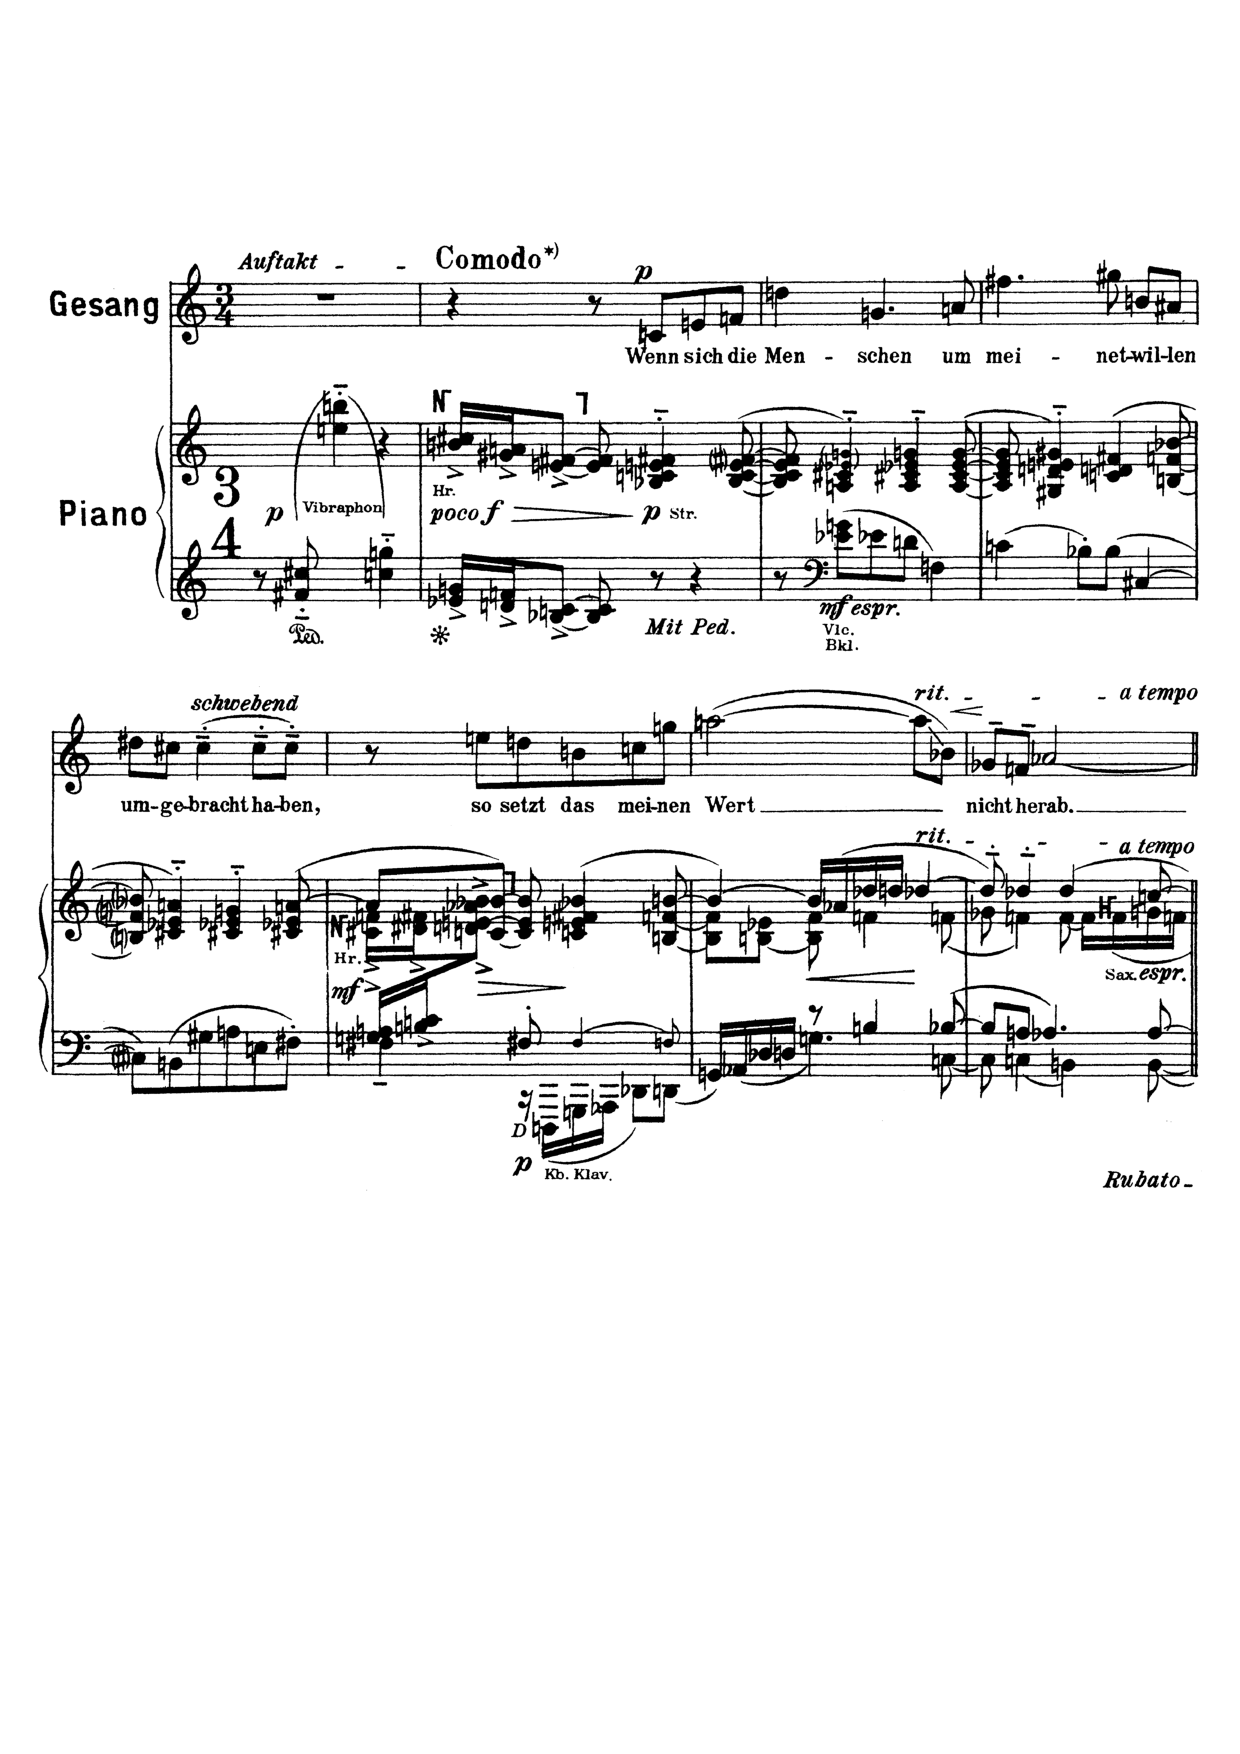
\includegraphics[width=6.5in]{figures/berg1.pdf}
	\caption[Berg's \emph{Lulu}]{Alban Berg's \emph{Lulu} \cite[182]{Starr1984}.}
	\label{fig:berg-lulu}
\end{figure}

%--------------------------------------------------------------------------
\section{Basic Derivation Techniques}

Derivation is the process of extracting ordered segments from rows in order to generate new compositional materials. It is a technique that dates back to the Second Viennese School. In its most incipient form, a composer may simply extract these segments from a row, and combine them to form another, as seen in Berg's \emph{Lulu}. The basic row used by Berg is $S = \{ 10, 2, 3, 0, 5, 7, 4, 6, 9, 8, 1, 11 \}$. In the Prologue, however, one is greeted with the row $\{ 10, 3, 4, 9, 2, 7, 8, 1, 0, 5, 6, 11 \}$, as depicted in Fig.~\ref{fig:berg-prologue}. It is clear that the segments that constitute the Prologue's row are ordered segments in the basic row form, and that there is no concern for the fact that one row cannot obtained from the other via row operations.

\begin{figure}[htbp]
    \centering
	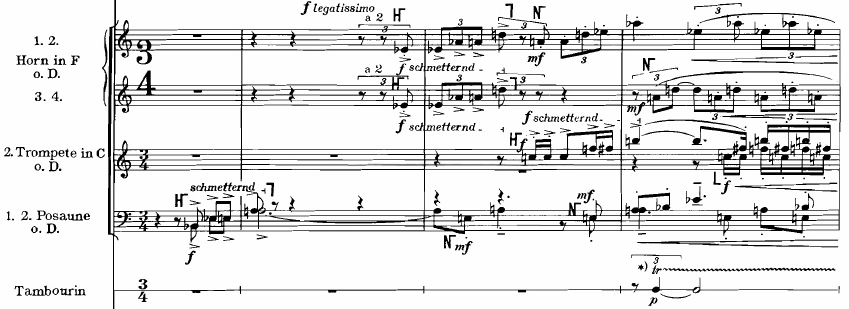
\includegraphics[width=6.5in]{figures/berg2.png}
	\caption[Derived Row in Berg's \emph{Lulu}]{Derived row in the \emph{Prologue} of Alban Berg's \emph{Lulu} \cite[182]{Starr1984}.}
	\label{fig:berg-prologue}
\end{figure}

More structured approaches to derivation often involve deriving a row from a combination matrix of rows. The rows combined in the matrix are usually twelve-tone transforms of the same basic row. The rows that are derived from the segments of these transforms may or may not be themselves transforms of the basic row. Ex.~\ref{ex:derivation} illustrates a very simple procedure for combining rows in a matrix to generate another.

%TODO: cite Morris here

\begin{example}
	\label{ex:derivation}
	The basic row in \emph{Lulu} may be used as motivation for a basic derivation procedure. The first step is to create a $2 \times 24$ array where the first row is $S$ followed by $\R(S)$, and the second row is initially undefined.
	\begin{equation}
    	\left[
    	\begin{array}{cccccccccccc|cccccccccccc}
        	10 & 2 & 3 & 0 & 5 & 7 & 4 & 6 & 9 & 8 & 1 & 11 & 11 & 1 & 8 & 9 & 6 & 4 & 7 & 5 & 0 & 3 & 2 & 10 \\
        	. & . & . & . & . & . & . & . & . & . & . & . & . & . & . & . & . & . & . & . & . & . & . & .
    	\end{array}
    	\right] \enspace.
	\end{equation}
	Next, an arbitrary segment is chosen, separated from the the top row, and placed in in the bottom row:
	\begin{equation}
    	\left[
    	\begin{array}{cccccccccccc|cccccccccccc}
        	. & 2 & 3 & . & . & . & 4 & 6 & 9 & 8 & 1 & 11 & . & . & . & . & . & . & 7 & 5 & 0 & . & . & 10 \\
        	10 & . & . & 0 & 5 & 7 & . & . & . & . & . & . & 11 & 1 & 8 & 9 & 6 & 4 & . & . & . & 3 & 2 & .
    	\end{array}
    	\right] \enspace.
	\end{equation}
	Let $V = \{ 2, 3, 4, 6, 9, 8, 1, 11, 7, 5, 0, 10 \}$. Then $V$ is a row derived from $S$. In particular, the ordered segment $\{ 10, 0, 5, 7 \}$ in $S$ is preserved by $\R(V)$, and a counterpoint that combines $S$ vertically with $V$ horizontally is possible by construction.
\end{example}

It is of interest to note at this point that, in this kind of construction, the choice of a particular segment is already an important compositional decision. This choice bears relevance in that it establishes motivic material, that is, the segment itself. It also potentially introduces complementary harmonic regions, one given by the segment, the other given by its set complement. Moreover, and perhaps more importantly, it presents an opportunity for exploring syntax. There are a multitude of ways in which a composer may obtain syntax from a simple derivation procedure such as the one given in Ex.~\ref{ex:derivation}. One way would be to find an operation that makes the chosen segment invariant. In particular, it is easily checked that $S_1 = \{ 10, 0, 5, 7 \} = \R\T_5\I(S_1)$. Ex.~\ref{ex:derivation} can then be extend into the combination array $[S \; | \; \R(S) \; | \; \R\T_5\I(S) \; | \; \T_5\I(S_1)]$. In the extended array, the segment $S_1$ would be preserved, but the row derived from $\R\T_5\I(S)$ would not be a transform of $V$. If the set complement of $S_1$ in $V$ were parsed to produce more than one harmonic region, then the complement of $S_1$ under this newly derived row would produce different harmonic regions. This procedure can be very pertinent compositionally, as it would be capable of producing contrasting harmonic regions while maintaining motivic coherence under the $S_1$ segment.

Yet another way of generating syntax from derivation would be to follow $S$ with $V$ itself. A new row would then be derived from $V$, say $Q$, and eventually $V$ would be follow with $Q$. Repeating this procedure \emph{ad libitum} could generate many contrasting harmonic regions. In particular, this type of derivation is seen in Donald Martino's \emph{Notturno} of 1974, a composition that won the Pulitzer Prize in the following year \cite[181]{Starr1984}. If, by compositional choice, the chain of derived rows picked always the same order numbers, then a potential for rhythmic and agogic coherence could also be explored.

%TODO: add Schoenberg Quartet 4 example here

%--------------------------------------------------------------------------
\section{The early work of Donald Martino}

The beginnings of derivation techniques can be traced back to Donald Martino's \emph{The Source Set and Its Aggregate Formations} \cite{Martino1961}, a paper whose main purpose is another, namely to generalize the construction of columnar realizations, although this latter term appears to have been coined by \cite{Starr1984}. The techniques employed by Martino are heavily influenced by Babbitt's ideas on combinatoriality \cite[224]{Martino1961}, and make extensive use of tables. Below is a fragment of the source hexachords table given in \cite[229]{Martino1961}. The author, in the interest of generalizing the procedure, provides also trichordal, tetrachordal, and even pentachordal combinatoriality tables, as well as a somewhat brief discussion on uneven partitions of a row and their combinatoriality implications \cite[267]{Martino1961}.

\begin{table}[htbp]
    \caption[Martino's Source Hexachords]{Fragment of a table for consulting source hexachords in \cite[229]{Martino1961}.}
    \centering
    \vspace{12pt}
    \begin{tabular}{c|cccccc}
        \hline\\
        No. & Set & Interval Vector & TTO's \\\\
        \hline\\
        A1 & $\{0,1,2,3,4,5\}$ & $\langle 5,4,3,2,1,0 \rangle$ & $\{\T_6,\T_{11}\I,\R\T_{11},\R\T_6\I\}$ \\\\
        B2 & $\{0,2,3,4,5,7\}$ & $\langle 3,4,3,2,3,0 \rangle$ & $\{\T_6,\T_{1}\I,\R\T_{1},\R\T_6\I\}$ \\\\
        3 & $\{0,1,3,4,5,8\}$ & $\langle 3,2,3,4,3,0 \rangle$ & $\{\T_6,\R\T_2\}$ \\\\
        E4 & $\{0,1,4,5,8,9\}$ & $\langle 3,0,3,6,3,0 \rangle$ & $\{\T_{2,6,10},\T_{3,7,11}\I,\R\T_{3,7,11},\R\T_{2,6,10}\I\}$ \\\\
        C5 & $\{0,2,4,5,7,9\}$ & $\langle 1,4,3,2,5,0 \rangle$ & $\{\T_6,\T_{3}\I,\R\T_{3},\R\T_6\I\}$ \\\\
        \hline
    \end{tabular}
\end{table}

Martino acknowledges the aggregates formed by combinatoriality are not necessarily ordered \cite[228]{Martino1961}, rather seeing it from the bright side of diversity, in which the set union of a columnar aggregate being capable of \emph{deriving} a different row class is actually more appealing than self-similarity, which is not at all considered. The same passage brings, to our knowledge, the first \emph{explicit} mention in the literature of a technique for deriving new rows from columnar aggregates in more generality than what what is seen in Schoenberg's fourth string quartet. This technique is reproduced below in \ref{ex:martino-derivation}. In mentioning derivation, Martino juxtaposes it to another way, in his view, of progressing through hexachords, namely the \emph{fragmentation} or partitioning of the original series, ultimately deeming both procedures essentially the same, as derivation via aggregate realizations can surely be seen as the fragmentation of the (new) series obtained vertically.

\begin{example}
	\label{ex:martino-derivation}
	\cite[231]{Martino1961}
	Let $S = \{ 0, 4, 11, 3, 1, 2, 5, 6, 9, 8, 10, 7 \}$ and consider the trivial combination matrix given below.
	\begin{equation}
    	\hat{A} = [\hat{A}_1 | \hat{A}_2 | \hat{A}_3 | \hat{A}_4] = \left[
    	\begin{array}{ccc|ccc|ccc|ccc}
        	0 & 4 & 11 & 3 & 1 & 2 & 5 & 6 & 9 & 8 & 10 & 7 \\
        	7 & 10 & 8 & 9 & 6 & 5 & 2 & 1 & 3 & 11 & 4 & 0
    	\end{array}
    	\right] \enspace.
	\end{equation}
	In particular, the hexachords given by $\hat{A}_i$ can be combined with their transforms under $\T_1\I$, yielding the following matrix:
	\begin{equation}
    	A = [A_1 | A_2 | A_3 | A_4] = \left[
    	\begin{array}{ccc|ccc|ccc|ccc}
        	0 & 4 & 11 & 3 & 1 & 2 & 5 & 6 & 9 & 8 & 10 & 7 \\
        	7 & 10 & 8 & 9 & 6 & 5 & 2 & 1 & 3 & 11 & 4 & 0 \\
        	\hline
        	1 & 9 & 2 & 10 & 0 & 11 & 8 & 7 & 4 & 5 & 3 & 6 \\
        	6 & 3 & 5 & 4 & 7 & 8 & 11 & 0 & 10 & 2 & 9 & 1
    	\end{array}
    	\right] \enspace.
	\end{equation}
	Transforms of the row $Q = \{ 7, 0, 10, 6, 4, 1, 3, 5, 8, 9, 2, 11 \}$ can then \emph{almost} be derived from the columns of $A$, except for a single symmetry between pitch-classes 6 and 5, as seen below.
	\begin{equation}
        \left[
        \begin{array}{cccccccccccc|cccccccccccc}
            & 0 &&& 4 &&&&&&& 11 &&&& 3 & 1 &&& 2 &&&& \\
            7 && 10 &&&&&& 8 &&& && 9 &&&&&&& \boxed{6} & \boxed{5} && \\
            \hline
            &&&&& 1 &&&& 9 & 2 & &&&&&& 10 & 0 &&&& 11 & \\
            &&& 6 &&& 3 & 5 &&&& & 4 && 7 &&&&&&&&& 8
        \end{array}
        \right. \cdots
    \end{equation}
    This apparent failure did not seem to bother Martino at all, as his focus remained in establishing a concrete foundation for combinatoriality. In order to extend the above procedure to eight rows of counterpoint, some adjustments must be made, namely columnar aggregates are needed whose rows are allowed to have different numbers of elements, as shown below. This second folding is otherwise accomplished much the same way, by choosing a hexachord from $A_1$, and determining its combinatoriality properties via table lookup.
    \begin{equation}
    	\left[
    	\begin{array}{cc|cc|cc|cc|}
        	0 & 4 & 11 && 3 & 1 & 2 & \\
        	7 & 10 & 8 && 9 && 6 & 5 \\
        	1 && 9 & 2 & 10 && 0 & 11 \\
        	6 && 3 & 5 & 4 & 7 & 8 & \\
        	2 && 6 & 1 & 5 && 3 & 4 \\
        	9 && 0 & 10 & 11 & 8 & 7 & \\
        	3 & 11 & 4 && 0 & 2 & 1 & \\
        	8 & 5 & 7 && 6 && 9 & 10
    	\end{array}
    	\right. \cdots
	\end{equation}
\end{example}

It is easy to understand why Martino was so motivated by creating as much diversity as possible from a single row in a structured manner. If not because creating variation upon some fixed foundation has been a constant in music composition since Bach, serialism up to that point had seen countless pieces in which the very same series was presented over and over again, frequently in the same $\R\T_n\I$ form for entire passages. As innovative as it is, not even the first movement of Schoenberg's fourth string quartet escapes this paradigm. The idea of having a systematic approach to syntactically moving from one row class to another, although latent in late Schoenberg, ultimately defines one of the most remarkable trends in the next chapter of serialism. Martino actually manages to solve both problems at once with derivation, as it gives the composer the opportunity to focus on the derived rows, while using a somewhat more abstract row to generate syntax, even though this potential is only explored in his later pieces, and not quite yet in \cite{Martino1961}. For now, what is most important is to derive as much harmonic diversity as possible from the rigidity of an omnipresent series.

Ex.~\ref{ex:oblique} illustrates the tetrachordal case of a technique described in \cite[241]{Martino1961} as \emph{oblique combination}, although other cases, including those where the overlap occurs at unequal partitionings of the row are considered. Oblique combinations are seen as special, yet straightforward cases of other types of combinatoriality \cite[267]{Martino1961} than hexachordal.

\begin{example}
	\cite[241]{Martino1961}
	\label{ex:oblique}
	Let $S = S_1 | S_2 | S_3$ be a twelve-tone row, partitioned into tetrachords. Let $f$ and $g$ be TTO's, and considered the following oblique combination matrix:
	\begin{equation}
    	\left[
    	\begin{array}{c|c|c|c|c}
        	S_1 & S_2 & S_3 & . & . \\
        	. & f(S_3) & f(S_2) & f(S_1) & . \\
        	. & . & g(S_1) & g(S_2) & g(S_3)
    	\end{array}
    	\right] \enspace.
	\end{equation}
	It follows:
	\begin{enumerate}[i.]
		\item If $S_1 = \T_i\I(S_1)$ \emph{only} for some $i$, then $f = \R\T_j$ for some $j$, and $g = \T_k\I$ for some $k$;
		\item If $S_3 = \T_i\I(S_3)$ \emph{only} for some $i$, then $f = \R\T_j\I$ for some $j$, and $g = \T_k$ for some $k$;
		\item If $S_1 = \T_i\I(S_1)$ \emph{only} for some $i$ and $S_3 = \T_j\I(S_3)$ for some $j$, then $f = \R\T_k\I$ for some $k$, and $g = \T_\ell\I$ for some $\ell$;
		\item If $S_1 = \T_i\I(S_1)$ \emph{only} for some $i$, $S_3 = \T_j\I(S_3)$ for some $j$, and $S_1 = \T_k(S_3)$ for some $k$, then $f = \T_\ell\I$ or $f = \R\T_\ell\I$ for some $\ell$, and $g = \T_m\I$ or $g = \R\T_m\I$ for some $m$;
		\item If $S_1 = \T_i(S_3)$ \emph{only} for some $i$, then $f = \T_j$ or $f = \R\T_j$ for some $j$, and $g = \T_k$ or $g = \R\T_k$ for some $k$;
		\item If $S_3 = \T_i\I(S_1)$ \emph{only} for some $i$, then $f = \T_j\I$ or $f = \R\T_j$ for some $j$, and $g = \T_k$ or $g = \R\T_k\I$ for some $k$.
	\end{enumerate}
\end{example}

%TODO: finish Martino

%--------------------------------------------------------------------------
\section{The set-theoretic view of Daniel Starr}

In one of the seminal academic works in the field of twelve-tone theory, \cite{Starr1984} utilizes a mostly set-theoretic framework to understand and categorize rows and procedures involved in producing derivation, polyphony, and self-derived combination matrices. This set-theoretic approach revolves around the idea of looking at collections from the standpoint of their order constraints: a totally constrained set with no precedence contradictions is a twelve-tone row; a completely unconstrained set of twelve tones represents the free aggregate; a maximally constrained one is what the author calls the simultaneous aggregate, that is, a twelve-tone cluster. Sets that live in-between can often be projected in the middle and background of a composition, fact that amounts to a Schenkerian-flavored view of the whole process.

Mathematically, the ideas in \cite{Starr1984} translate into considering the set $U$ of all ordered pairs of pitch classes. There are twelve choices for the first position, and twelve choices for the second position. As both choices are independent, this set has cardinality $12^2 = 144$. An element of $U$ is called an order constraint, and a subset $C$ of $U$ is called a pitch-class relation. The latter can be viewed as a $12 \times 12$ matrix where the entry $c_{ij}$ is equal to one whenever $\{ i, j \} \in C$, and zero otherwise. One can then apply bitwise operations to these matrices in a very computationally efficient manner: bitwise \emph{and} and \emph{or} correspond respectively to set intersection and union. For any pair of pitch classes $x$ and $y$, define a relation $x \sim y$ on the power set of $U$ by the set inclusion of the element $\{ x, y \}$. A subset $C$ will then be reflexive if, whenever an element of $C$ (which is a set) contains the pitch class $x$, then $\{ x, x \} \in C$. In words, reflexivity means that if a reflexive collection $C$ of notes contains an element $x$, then $x$ precedes (and follows) itself in $C$. The free aggregate is a minimal reflexive subset of $U$ that contains all twelve tones. The relation $\sim$ will be symmetric if $\{ x, y \} \in C$ implies $\{ y, x \} \in C$, and antisymmetric whenever $\{ x, y \} \in C$ implies $\{ y, x \} \notin C$, for $x \ne y \in \mathbb{Z}/ 12 \mathbb{Z}$. Similarly, transitivity is defined as $\{ x, y \} \in C$ and $\{ y, z \} \in C$, then $\{ x, z\} \in C$; and trichotomy is defined as either $\{ x, y \} \in C$ or $\{ y, x \} \in C$ for any $x \ne y \in \mathbb{Z}/ 12 \mathbb{Z}$. The relation $\sim$ is, of course, an order relation on the set of twelve tones by definition. A partial order is one that is reflexive, transitive, and antisymmetric, while a total order (a row), is a partial order that satisfies trichotomy.

Often, pitch-class relations will contain many redundancies due to transitivity. In order to express these relations as oriented graphs, such redundancies must first be removed, or pruned. This process can be reversed and a pitch-class relation can be extended to the point of its transitive closure. It is also common for a pitch-class relation to be absent of any order constraint involving both $\{ x, y \}$, in which case $x$ and $y$ are said to be incomparable. Such $x$ and $y$ are bound to be struck together, or else be \emph{linearized} by the injection of some constraint that will make them comparable, as long as there still remains a partial order, that is, as long as this process does not introduce a symmetry, for instance. The set of all total orderings that can be linearized from some partial order is called its total order class. In a completely analogous manner, a pitch-class relation can be can \emph{verticalized} by removing constraints, and again minding that the result is still transitive and symmetric. A partial order covers another whenever the former is a verticalization of the latter. A simple procedure to guarantee that a verticalization will remain a partial order is to take its union with the free aggregate, then subject this union to an extension operation, thus providing reflexivity in the first step, as well as transitivity in the second. The following can be said about covering, and about unions and intersections of pitch-class relations:

\begin{theorem}
    \cite[193]{Starr1984}
    \begin{enumerate}[i.]
        \item Covering is transitive;
        \item A pitch-class relation is covered by its extension;
        \item If a pitch-class relation covers another, then the extension of the former covers the extension of the latter.
    \end{enumerate}
\end{theorem}

\begin{theorem}
    \cite[194]{Starr1984}
    \label{starr-theorem}
    Let $A$ and $B$ be partial orders and denote by $\Toc(A)$ and $\Toc(B)$ their respective total order classes. Then
    \begin{equation}
        \Toc(A) \cap \Toc(B) = \Toc(\Ext(A \cup B)) \enspace,
    \end{equation}
    where $\Ext$ is the extension operator. Moreover, if $A_i$ is a finite sequence of $n$ partial orders, then
    \begin{equation}
        \bigcap_{i = 0}^{n} \Toc(A_i) = \Toc \left[ \Ext\left ( \bigcup_{i = 0}^{n} A_i \right) \right] \enspace.
    \end{equation}
\end{theorem}

\begin{theorem}
    \cite[194]{Starr1984}
    The intersection of two partial orders is again a partial order.
\end{theorem}

Th.~\ref{starr-theorem} will play a crucial role in the development of derivation techniques. Of vital importance is the fact that one can operate on pitch-class relations the same way one operates on pitch-class sets:

\begin{theorem}
    \cite[195]{Starr1984}
    Let $C$ be a pitch-class relation and $\{ a, b \}$ an element of $U$ such that $\{ a, b \} \in C$.
    \begin{enumerate}[i.]
        \item If $F$ is a pitch-class operation, then $\{ F(a), F(b) \} \in F(C)$ if and only if $\{ a, b \} \in C$. In particular, if $\R(C)$ is the retrograde of $C$, then $\{ a, b \} \in \R(C)$ if and only if $\{ b, a \} \in C$.
        \item If $C$ is totally ordered, then $\R(C) = (S \setminus D) \cup F$, where $S$ is the simultaneous aggregate and $F$ is the free aggregate.
        \item If $C_1$ covers $C_2$, then $F(C_1)$ covers $F(C_2)$.
        \item Finally, if $C$ is $F\R$-invariant, then all cycles in $F$ have length two.
    \end{enumerate}
\end{theorem}

\emph{Aggregate realizations} are an important concept defined in \cite[197]{Starr1984}, which lead to a classification of partial orders, as well as to many musical applications. An aggregate realization is a particular type of partial order $C$ in which, for any pair of pitch classes $a, b$, if $a$ and $b$ are incomparable in $C$, then the set of pitch classes that precede $a$ in $C$ is equal to the set of pitch classes that precede $b$ in $C$, and also the set of pitch classes that follow $a$ in $C$ is equal to the set of pitch classes that follow $b$ in $C$. Aggregate realizations arise naturally from a total order in the sense that they belong to the set of all partial orders that are covered by said total order. An interesting compositional application of aggregate realizations is that of projecting a total order as a middle-ground entity.

\begin{example}
    \cite[197]{Starr1984}
    Given a sequence $S$ of partial orders, all of which covered by the same total order, say $X$, if both $X$ is never stated in the foreground and $S$ contains all order constraints in $X$, then a musical passage in which $S$ is stated in the foreground will bear $X$ as a middle-ground entity. In the case where $S$ does not comprise all the order constraints in $X$, some other partial order that covers $S$ will be projected in the middle-ground. In the particular case where a composer is dealing with pitch classes, projecting a partial order is equivalent to inducing the listener to infer its order constraints. If, in this case, two pitch classes are incomparable, then they are bound to be struck together.
\end{example}

The concept of a \emph{row segment}, which is fairly straightforward in twelve-tone theory, has an analogue in \cite[198]{Starr1984}, where it is defined as a pitch-class relation that is reflexive, transitive, and antisymmetric, with the additional requirement that some subset of its order constraints also satisfy trichotomy. Arguably more important is the concept of an \emph{embedded segment}. For any partial order that covers some row segment, that segment is said to be an embedded segment of the partial order. By transitivity of covering, any other partial order covering the former partial order will have the aforementioned row segment embedded in it, including naturally any total order in its total order class. In this sense, a partial order may be seen as the union (possibly the extension) of its various embedded segments:

\begin{example}
    \label{starr-common-tones}
    \cite[200]{Starr1984}
    Consider two total orders $X = \{ 0, 1, 7, 2, 10, 9, 11, 4, 8, 5, 3, 6 \}$ and $Y = \{ 1, 2, 8, 3, 11, 10, 0, 5, 9, 6, 4, 7 \}$ where, in particular, $Y = \T_1(X)$. Seen as total orders, take the intersection $X \cap Y$, then prune it. This process yields a graph whose longest row segments are $\{ 1, 2, 10, 9, 4 \}$, $\{ 1, 2, 10, 5, 6 \}$, $\{ 1, 2, 11, 5, 6 \}$, $\{ 1, 2, 8, 5, 6 \}$, and $\{ 1, 2, 8, 3, 6 \}$. These row segments are, in turn, the longest that are embedded segments of both $X$ and $Y$.
\end{example}

It is interesting to point out that the procedure described in Ex.~\ref{starr-common-tones} is in fact an algorithm to find common tones under transposition, and can be extended to any other pitch-class operation. Th.~\ref{rahn-common-tone} describes a well-known technique of simply \emph{counting} common tones.

\begin{theorem}
	\label{rahn-common-tone}
	\cite[10]{Rahn1975}
	The number of common tones between a set $S$ and some transposition of itself is given by
	\begin{equation}
		|S \cap \T_n(S)| = |\{x - y = n : x, y \in S\}| \enspace.
	\end{equation}
	The number of common tones between a set $S$ and some inversion of itself is given by
	\begin{equation}
		|S \cap \T_n\I(S)| = 2 \cdot |\{x + y = n : x, y \in S\}| + |\{a \in S : 2a = n\}| \enspace.
	\end{equation}
	Moreover, the cardinality of the set $\{a \in S : 2a = n\}$ is at most 2.
	\begin{proof}
		The occurrences of pairs of pitch classes that are interchanged by the operation at hand must be counted and doubled, for if $x$ maps onto $y$ under some $\T_n\I$, then certainly $y$ maps onto $x$ under the same operation, given that every inversion operation has order two. In addition to that, the occurrences of pitch classes that may map onto themselves under the aforementioned operation must be accounted for. For any pair $a \ne b \in S$, it follows $a$ and $b$ are exchanged by some operation $\T_n\I$ whenever both $\T_n\I(a) = b$ and $\T_n\I(b) = a$ hold. Since $\T_n\I(a) = -a + n$, and similarly $\T_n\I(b) = -b + n$, if the pair is exchanged, then both $-a + n = b$ and $-b + n = a$ must be true. Adding the last two expressions and solving for $n$ yields $a + b = n$, which is the first set in the right-hand side of the formula. As discussed above, the cardinality of this set must be doubled. For any $a$, it follows that $\T_n\I(a) = a + n$, hence $a = \T_n\I(a) \iff a = -a + n$, that is, whenever $2a = n$. That is the second set in the formula. Finally, for any pair $(a, n)$ such that $a = \T_n\I(a)$, it also follows that $a + 6 = -(a + 6) + n \iff 2a = n$, so that $a + 6 = \T_n\I(a + 6)$ by the above. Thus the set $\{a \in S : 2a = n\}$ has cardinality at most 2, proving the last assertion.
	\end{proof}
\end{theorem}

\begin{example}
    \label{rahn-example}
    \cite[11]{Rahn1975}
    Write $S = \{ 0, 1, 4, 5, 8, 9 \}$ and consider some inversion operation. An application of Th.~\ref{rahn-common-tone} yields the table below.
    \begin{table}[htbp]
    \caption[Rahn's Common Tones Under Inversion]{Common tones under inversion between $S = \{ 0, 1, 4, 5, 8, 9 \}$ and itself.}
    \centering
    \vspace{12pt}
    \begin{tabular}{ c | *{12}{c} }
        \hline\\
        $n$ & 0 & 1 & 2 & 3 & 4 & 5 & 6 & 7 & 8 & 9 & 10 & 11 \\
        $2 \cdot |\{x + y = n : x, y \in S\}|$ & 2 & 6 & 2 & 0 & 2 & 6 & 2 & 0 & 2 & 6 & 2 & 0 \\
        $|\{a \in S : 2a = n\}|$ & 1 & 0 & 1 & 0 & 1 & 0 & 1 & 0 & 1 & 0 & 1 & 0 \\
        \hline\\
        Total & 3 & 6 & 3 & 0 & 3 & 6 & 3 & 0 & 3 & 6 & 3 & 0 \\
        \hline
    \end{tabular}
    \end{table}
\end{example}

\begin{example}
	Ex.~\ref{rahn-example} and the omitted proof of \ref{rahn-common-tone} under transposition can be demonstrated in a much simpler way by observing the cycle decomposition of each operation at hand. If $n = 3$, then
	\begin{equation}
		\T_3\I = (0 \; 3) (1 \; 2) (4 \; 11) (5 \; 10) (6 \; 9) (7 \; 8) \enspace.
	\end{equation}
	Hence, under $\T_3\I$, every pitch-class in $S = \{ 0, 1, 4, 5, 8, 9 \}$ maps to the complement of $S$. If the operation is, for instance, $\T_9$, then since
	\begin{equation}
		\T_9 = (0 \; 9 \; 6 \; 3) (1 \; 10 \; 7 \; 4) (2 \; 11 \; 8 \; 5) \enspace,
	\end{equation}
	it follows $S = \{ 0, 1, 4, 5, 8, 9 \}$ shares three common tones with $\T_9(S)$, namely $0 \mapsto 9$, $4 \mapsto 1$, and $8 \mapsto 5$.
\end{example}

In practice, however, many composers choose to compute common tones by writing down an entire matrix. This procedure has the advantage of, not only giving all indices of transposition under which a set shares common tones with itself or other set, but it is also possible to determine whether these common tones will preserve their ordering after the transform by examining the matrices' diagonals.

\begin{example}
	\cite[49]{Morris1987}
    \label{morris-common-tones}
    Let $X$ be an $n$-tone row seen as a column vector, and consider the $n \times n$ matrix $A = [X, \cdots, X]$. In particular, the matrix $B = A - A^T$ will have a main diagonal of zeros, which indicates that $X$ shares with itself $n$ common tones under $T_0$. If there are $k$ threes in the matrix, then $X$ will share with itself $k$ tones under $T_3$. There is no requirement that a row be compared with itself. If, for instance, $A$ is given as above, and $\bar{A}$ is the matrix for the row $\bar{X}$, then counting the number $k$ of, say, threes in $B = A - \bar{A}^T$, will mean in turn that $X$ and $\T_3(\bar{X})$ share $k$ tones under $\T_3$. Naturally, the main diagonal of $B$ will not comprise only zeros if $A \ne \bar{A}$. To find common tones under inversion, let $B = A + A^T$ and, similarly, $\M$ and $\M \circ \I$ become $B = A - \M(A)^T$ and $B = A + \M(A)^T$. Finally, if the indices being counted are disposed in any of the matrix's diagonals, then they will preserve ordering after the transform, thus becoming embedded segments; if, in addition, they are adjacent, then they will in fact be row segments shared by $X$ and the transform of $\bar{X}$.
\end{example}

The matrix for finding common tones under transposition that is described in Ex.~\ref{morris-common-tones} has the interesting property that it becomes a symmetric matrix when $A = \bar{A}$ and its elements are taken as interval classes. This reflects the fact that, if $X$ shares $k$ tones with $T_i(X)$, then surely $T_i(X)$ will share exactly $k$ tones with $T_{12 - i}(X)$. If $i$ is an interval class, then $i = 12 - i$, showing why the matrix will be symmetric. The matrix of common tones under inversion is always symmetric, regardless whether its elements are taken as interval classes. For multiplicative operations, however, will often lack multiplicative inverses in twelve tones. For $p$-TET systems where $p$ is prime, multiplicative operations yield symmetric matrices as well, but those will sometimes require a proper definition of multiplicative interval classes.

The importance of the procedure described in Ex.~\ref{starr-common-tones} is due to the fact that the technique in Ex.~\ref{morris-common-tones} can only go as far as counting the number of common tones, whereas the former procedure can actually tell \emph{what} these common tones are in a more straightforward manner. In addition, it can be very computationally effective if the rows being compared are written as binary square matrices describing their order constraints. Taking then their intersection is easy, since binary operations can be used efficiently for this type of matrix. Pruning, if expressing the result as a graph, is also fast and simple \cite[200]{Starr1984}. In a completely analogous manner to the principle of pulling row segments from a series, row segments can be concatenate in order to formulate a new series. 

\begin{example}
    \cite[200]{Starr1984}
    Let $X = \{ 0, 1, 2 \}$ and $Y = \{ 3, 4, 5 \}$ be row segments such that $X \cap Y = \emptyset$ when seeing $X$ and $Y$ as partial orders. The concatenation $X | Y$ will then be the partial order:
    \begin{equation}
        X \cup Y \cup \{ \{ a, b \} : a \in X, b \in Y \} \enspace.
    \end{equation}
    It follows immediately that both $X$ and $Y$ are embedded row segments of $X | Y$. Note that the use of concatenation here is sequential, that is, the entire row segment $X$ precedes the entire row segment $Y$ in $X | Y$. In other words, intercalation of segments are not allowed when concatenating.
\end{example}

Whereas aggregate realizations correspond to a totally ordered sequence of disjoint subsets of the free aggregate, a \emph{columnar aggregate} is, on the other hand, a set of disjoint row segments where, even though the internal order of each segment is total, all segments are pairwise incomparable \cite[201]{Starr1984}. In addition, a columnar aggregate must contain the free aggregate as a subset, so that all pitch classes belonging to a given base are included in every column. This is essentially a combination matrix in twelve-tone theory.

\begin{example}
    \cite[201, 210]{Starr1984}
    The intersection of the set of all aggregate realizations with the set of all columnar realizations contains the set of all total orders (and thus all row segments), as well as the free aggregate. A total order is trivially an aggregate realization, and it is trivially a columnar realization. Any total order contains the free aggregate by the above.
\end{example}

The procedure described in Ex.~\ref{ex:derivation} represents a type of derivation in which the series being displayed vertically is unrelated to the series being derived horizontally, except for the fact that both share a row segment when one of the rows is retrograded. The construction is part of a more general procedure, detailed in in \cite[211]{Starr1984}, in which a row is always matched with a retrograded transform of itself. In the particular case of Ex.~\ref{ex:derivation}, the transform, say $F$, was $\T_0$ for simplicity, but arbitrary pitch-class operations may be used. Denote the given series by $S$, and define similarly the derived row as $V = V_1 | V_2$, that is, $V$ is a concatenation of two row segments. The only requirement is that $V_1$, the segment that is singled out, remain invariant under $F$, which will force $V_2$ to also be invariant under $F$. In Ex.~\ref{ex:derivation} this requirement is satisfied trivially. The generealized procedure is given schematically in Table~\ref{derivation-retrograde}.

\begin{table}[htbp]
	\cite[212]{Starr1984}
    \caption[Derivation Involving the Retrograde and an Arbitrary Operation]{Schematics of a derivation procedure involving the retrograde and an arbitrary operation $F$.}
    \label{derivation-retrograde}
    \centering
    \vspace{12pt}
    \begin{tabular}{c|cc}
        \hline\\
        & $S$ & $\R \circ F(S)$ \\
        \hline\\
        $V$ & $V_1$ & $V_2$ \\
        $\R \circ F(V)$ & $\R \circ F(V_2)$ & $\R \circ F(V_1)$ \\
        \hline
    \end{tabular}
\end{table}

Ex.~\ref{ex:derivation-ordered} illustrates a derivation procedure similar to that in Ex.~\ref{ex:derivation} where the operation $F$ is not trivial. It also features an application of the technique described in Ex.~\ref{morris-common-tones} for finding common row segments.

\begin{example}
    \label{ex:derivation-ordered}
    Let $S = \{ 10, 2, 3, 0, 5, 7, 4, 6, 9, 8, 1, 11 \}$, the row in Berg's \emph{Lulu}, and consider the segment $\vec{s} = [10 \; 0 \; 5 \; 7]^T$ as a column vector. Now let $A^T = [\;\vec{s} \; | \; \vec{s} \; | \; \vec{s} \; | \; \vec{s}\;]$ be the square matrix whose every column is equal to $\vec{s}$. Then
	\begin{equation}
    	A + A^T = \begin{bmatrix}
    		2 & 10 & 3 & 5 \\
        	10 & 0 & 5 & 7 \\
        	3 & 5 & 10 & 0 \\
        	5 & 7 & 0 & 2
        \end{bmatrix} \pmod{12} \enspace.
	\end{equation}
	\noindent In particular, the row segment $\{ 10, 0, 5, 7 \}$ is invariant under $\R\T_5\I$, since $A + A^T$ displays an anti diagonal of fives. Thus, by matching $S$ with $\R\T_5\I(S)$, the row segment $\{ 10, 0, 5, 7 \}$ may be pbtained in the derived row $V$ itself, rather than in its retrograde, as was the case in Ex.~\ref{ex:derivation}. Setting it to $V_2$, say, yields $V = \{ 2, 3, 4, 6, 9, 8, 1, 11, 10, 0, 5, 7 \}$ and the combination matrix below:
	\begin{equation}
    	\left[
    	\begin{array}{cccccccccccc|cccccccccccc}
        	. & 2 & 3 & . & . & . & 4 & 6 & 9 & 8 & 1 & 11 & . & . & . & . & . & . & 10 & 0 & 5 & . & . & 7 \\
        	10 & . & . & 0 & 5 & 7 & . & . & . & . & . & . & 6 & 4 & 9 & 8 & 11 & 1 & . & . & . & 2 & 3 & .
    	\end{array}
    	\right] \enspace.
	\end{equation}
\end{example}

It is usually the case in this type of derivation that, unlike Ex.~\ref{ex:derivation-ordered}, the invariance of $V$ under $F$, or under $\R \circ F$ for that matter, does not preserve any ordering.

\begin{example}
    \cite[212]{Starr1984}
    Let $S = \{ 0, 1, 7, 2, 10, 9, 11, 4, 8, 5, 3, 6 \}$ and consider the operation
    \begin{equation}
        \T_2\I = (0 \; 2) (3 \; 11) (4 \; 10) (5 \; 9) (6 \; 8) \enspace.
    \end{equation}
    Upon inspection of the cycles of $\T_2\I$, that the segment $\{ 0, 1, 7, 2 \}$ is easily seen to be invariant under this operation. If a combination matrix involving $\R\T_2\I$ is considered, however, then the same ordered result as in Ex.~\ref{ex:derivation-ordered} shall not be obtained, since both $(1)$ and $(7)$ are fixed points. The same would happen to any $\T_k\I$ where $k$ is even. In particular, this shows that, in order to obtain the same ordered row segment in both columns of the combination matrix, $F$ cannot be trivial.
	\begin{equation}
    	\left[
    	\begin{array}{cccccccccccc|cccccccccccc}
        	0 & . & . & 1 & . & 7 & . & . & . & 2 & . & . & 10 & 9 & . & 11 & 4 & 8 & . & 5 & . & 3 & 6 & . \\
        	. & 8 & 11 & . & 9 & . & 6 & 10 & 3 & . & 5 & 4 & . & . & 0 & . & . & . & 7 & . & 1 & . & . & 2
    	\end{array}
    	\right] \enspace.
	\end{equation}
\end{example}

As a consequence of $F$ and the retrograde operation, combination matrices of this type feature two columns that are upside down $F$-mirrors of each other \cite[211]{Starr1984}. More can be said about such combination matrices. Proposition~\ref{derivation-polyphony-proposition} summarizes the general procedure under set-theoretic terms.

\begin{proposition}
	\label{derivation-polyphony-proposition}
    \cite[211, 214]{Starr1984}
    Consider a 2-row combination matrix $C$ where a row is derived via the retrograde and some operation $F$. Denote the derived row by $V = V_1 | V_2$. Then the first column is the partial order $C_1 = V_1 \cup \R \circ \F(V_2)$, and similarly the second column is the partial order $C_2 = V_2 \cup \R \circ \F(V_1)$, such that $C_2 = \R \circ F(C_1)$. If $D$ is a partial order that covers $C_1$, then $\R \circ F(D)$ will cover $C_2$, and if $D$ is in the total order class of $C_1$, that is, $D$ is a row that can be linearized from $C_1$, then $\R \circ F(D)$ is in the total order class of $C_2$. Finally, 2-row derivations of this type exist for arbitrary rows.
\end{proposition}

A distinction is made in \cite[211, 214]{Starr1984} between derivation and \emph{polyphonyzation}. The former departs from a combination matrix of rows to infer a concatenation of rows that constitute the linearized result of flattening the combination matrix. The latter is the opposite concept, that is, given a concatenation of rows, a combination matrix is constructed such that each column breaks down the row at the top into disjoint ordered segments. Although differentiating between derivation and polyphonization is an important concept in the set-theoretic view of the problem, this paper shall not make that distinction. The term derivation will be used indiscriminately to both the breaking down of rows into contrapuntal combination matrices, and the flattening thereof.

A related technique involving greater than 2-row counterpoint is achieved by \emph{folding} a combination matrix \cite[215]{Starr1984}. The process is similar to first constructing a matrix of hexachordal combinatoriality in the traditional sense, that is, where hexachords are seen as tropes rather than as row segments, then deriving rows from this matrix using the techniques above. Let $S$ be a row whose first hexachord is invariant under the operation $G$. Consider a row $V = V_1 | V_2$ and an operation $F$ such that $S$ is in the total order order class of $V_1 \cup \R \circ \F(V_2)$. Then putting $S$ in counterpoint with $G(S)$, as well as deriving $V$ from $S | \R\circ F(S)$ yields the schematic representation in Table~\ref{derivation-folded}:

\begin{table}[htbp]
	\cite[215]{Starr1984}
    \caption[Folded Derivation Involving the Retrograde]{Schematics of a folded derivation procedure involving the retrograde.}
    \label{derivation-folded}
    \centering
    \vspace{12pt}
    \begin{tabular}{c|cc}
        \hline\\
        & $S$ & $\R \circ F(S)$\\
        \hline\\
        $V$ & $V_1$ & $V_2$ \\
        $\R \circ F(V)$ & $\R \circ F(V_2)$ & $\R \circ F(V_1)$ \\
        $\R \circ GF(V)$ & $\R \circ GF(V_2)$ & $\R \circ GF(V_1)$ \\
        $G(V)$ & $G(V_1)$ & $G(V_2)$ \\
        \hline\\
        & $G(S)$ & $\R \circ GF(S) = \R \circ FG(S)$ \\
        \hline
    \end{tabular}
\end{table}

It is argued without proof in \cite[215]{Starr1984} that, in the derivation procedure described in Table~\ref{derivation-folded}, vertically satisfying $G$ while horizontally satisfying $F$ implies $F$ and $G$ must commute. Ex.~\ref{derivation-folded} shows a musical application of folded derivation.

\begin{example}
    \cite[215]{Starr1984}
    \label{ex:derivation-folded}
    Let $S = \{ 0, 1, 11, 3, 8, 10, 4, 9, 7, 6, 2, 5 \}$ and consider the operation $\T_6$:
    \begin{equation}
        \T_6 = (0 \; 6) (1 \; 7) (2 \; 8) (3 \; 9) (4 \; 10) (5 \; 11) \enspace.
    \end{equation}
    Let $V_1 = \{ 1, 3, 8, 9, 7, 2 \}$. Since the unordered set $V_1$ is $T_6$-invariant, it follows $V_2 = \{ 11, 0, 10, 4, 5, 6 \}$ and the following combination matrix is obtained:
    \begin{equation}
        \left[
        \begin{array}{cccccccccccc|cccccccccccc}
            & 1 && 3 & 8 &&& 9 & 7 && 2 && 11 && 0 &&& 10 & 4 &&& 5 && 6 \\
            0 && 11 &&& 10 & 4 &&& 6 && 5 && 8 && 1 & 3 &&& 2 & 9 && 7 &  
        \end{array}
        \right] \enspace.
    \end{equation}
    Consider further the operation $\T_5\I$:
    \begin{equation}
        \T_5\I = (0 \; 5) (1 \; 4) (2 \; 3) (6 \; 11) (7 \; 10) (8 \; 9) \enspace.
    \end{equation}
    Then $S_1 = \{ 0, 1, 11, 3, 8, 10 \}$ maps to its complement under $\T_5\I$, so $S$ can be used in a combination matrix where $S$ is matched with its transform under $\T_5\I$ in the usual way, that is, in a matrix of hexachordal combinatoriality. Then the row $\T_5\I(V)$ can be derived from $\T_5\I(S)$. Since $\T_5\I$ commutes with $T_6$, as any pitch-class operation does, the following folded derivation is possible:
    \begin{equation}
        \left[
        \begin{array}{cccccccccccc|cccccccccccc}
            & 1 && 3 & 8 &&& 9 & 7 && 2 && 11 && 0 &&& 10 & 4 &&& 5 && 6 \\
            0 && 11 &&& 10 & 4 &&& 6 && 5 && 8 && 1 & 3 &&& 2 & 9 && 7 & \\
            \hline
            5 && 6 &&& 7 & 1 &&& 11 && 0 && 9 && 4 & 2 &&& 3 & 8 && 10 & \\
            & 4 && 2 & 9 &&& 8 & 10 && 3 && 6 && 5 &&& 7 & 1 &&& 0 && 11
        \end{array}
        \right] \enspace.
    \end{equation}
\end{example}

\cite[216]{Starr1984} provides an analogue to the technique of oblique combination described in \cite[241, 267]{Martino1961} in the context of folded derivation, denoted \emph{skewed polyphonization}. The procedure consists of shifting horizontally one of the two rows of the derivation matrix. Skewed polyphonizations may be equivalent to folding combination matrices that involve the retrograde, and there is no requirement that the combinatoriality be hexachordal. An interesting compositional application consists of matching altogether different foldings of a row, thus effectively bridging different derivations of the same generative material.

\begin{table}[htbp]
	\cite[216]{Starr1984}
    \caption[Skewed Polyphonization Involving the Retrograde]{Schematics of a skewed polyphonization procedure involving the retrograde. The asterisk indicates there is no requirement that the same row class be derived in both foldings, in which case $V$ would be replaced by some other row $V^*$ and $G$ could be the identity.}
    \label{derivation-shifted}
    \centering
    \vspace{12pt}
    \begin{tabular}{ c | c c c }
        \hline\\
        & $S$ & $\R \circ F(S)$ & \\
        \hline\\
        $V$ & $V_1$ & $V_2$ & \\
        $\R \circ F(V)$ & $\R \circ F(V_2)$ & $\R \circ F(V_1)$ & \\
        $\R \circ G(V)^*$ && $\R \circ G(V_2)^*$ & $\R \circ G(V_1)^*$ \\
        $GF(V)^*$ && $GF(V_1)^*$ & $GF(V_2)^*$ \\
        \hline\\
        && $GF(S)$ & $\R \circ G(S)$ \\
        \hline
    \end{tabular}
\end{table}

Ex.~\ref{ex:derivation-shifted} shows an application of skewed polyphonization where combinatoriality is not hexachordal, but both foldings derive different transforms of the same row \cite[216]{Starr1984}:

\begin{example}
    \cite[216]{Starr1984}
    \label{ex:derivation-shifted}
    Consider the row $S = \{ 0, 1, 7, 2, 10, 9, 11, 4, 8, 5, 3, 6 \}$ and the combination matrix given by $\R\T_{10}\I(S)$ against $\T_{11}(S)$:
    \begin{equation}
        \left[
        \begin{array}{cccccccc|cccccccc}
            4 && 7 && 5 && 2 && 6 & 11 & 1 & 0 & 8 & 3 & 9 & 10 \\
            11 & 0 & 6 & 1 & 9 & 8 & 10 & 3 && 7 && 4 && 3 && 5
        \end{array}
        \right]
    \end{equation}
    Deriving the row $V = V_1 | V_2 = \{ 1, 7, 2, 9, 8, 3 \} | \{ 4, 5, 6, 11, 0, 10 \}$ from $S | \R\T_{10}\I(S)$, and following the scheme in Table~\ref{derivation-shifted}, yields the following shifted derivation:
    \begin{multline}
        \left[
        \begin{array}{cccccccccccc|cccccccc|c}
            & 1 & 7 & 2 && 9 &&& 8 && 3 && 4 &&&& 5 &&&& 6 \\
            0 &&&& 10 && 11 & 4 && 5 && 6 & && 7 &&&& 2 && \\
            \hline
            &&&&&&&&&&&& & 0 & 6 & 1 && 8 &&& 7 \\
            &&&&&&&&&&&& 11 &&&& 9 && 10 & 3 &
        \end{array}
        \right. \cdots \\\\
        \cdots \left. \begin{array}{c|cccccccc|cccccccccccc}
            & 6 & 11 && 0 &&&& 10 &&&&&&&&&&& \\
            & && 1 && 8 & 3 & 9 & &&&&&&&&&&& \\
            \hline
            & 7 &&&& 3 &&& & 3 && 4 && 5 & 10 && 11 &&&& 9 \\
            3 &&& 4 &&&& 5 & && 6 && 1 &&& 0 && 7 & 2 & 8
        \end{array} \right] \enspace.
    \end{multline}
\end{example}

Self-derivation is discussed in \cite[217, 226]{Starr1984} and is seen from both the set-theoretic perspective, and from the standpoint of aggregate realizations. The only difference between self-derivation and the general case is that in combination matrices of self-derivation all row forms belong to the same row class, that is, all rows are $RT_nI$-transforms of the original row. The same applies to folded and skewed combination matrices of self-derivation. The general scheme for a two-row combination matrix of self-derivation involving the retrograde is given in Table~\ref{derivation-self}:

\begin{table}[htbp]
	\cite[219]{Starr1984}
    \caption[Self-Derivation Involving the Retrograde]{Schematics of a self-derivation procedure involving the retrograde.}
    \label{derivation-self}
    \centering
    \vspace{12pt}
    \begin{tabular}{c|cc}
        \hline\\
        & $G(S)$ & $\R \circ FG(S)$ \\\\
        \hline\\
        $S$ & $S_1$ & $S_2$ \\\\
        $\R \circ F(S)$ & $\R \circ F(S_2)$ & $\R \circ F(S_1)$ \\\\
        \hline
    \end{tabular}
\end{table}

It is stated without proof in \cite[217]{Starr1984} that the operations $F$ and $G$ in Table \ref{derivation-self} must commute. For this self-derivation on two-row counterpoint case, however, simple inspection of the examples that follow such statement already affords a counter-proof.

\begin{example}
	\label{topSquareSideExample}
    \cite[218]{Starr1984}
    Let $S = S_1 | S_2 = \{ 3, 8, 1, 0, 9, 6 \} | \{ 4, 7, 10, 5, 2, 11 \}$ and consider the operation $\T_9\I$:
    \begin{equation}
        \T_9\I = (0 \; 9) (1 \; 8) (2 \; 7) (3 \; 6) (4 \; 5) (10 \; 11) \enspace.
    \end{equation}
    In particular, both $S_1$ and $S_2$ are invariant under $\T_9\I$. What is certainly not obvious, is that $S$ and $\T_9\I(S)$ can be derived from a combination matrix where the first column is $\T_7(S)$ and the second is $\T_9\I \circ \R\T_7(S) = \R\T_2\I(S)$, as shown in the following self-derivation matrix:
    \begin{equation}
    	\label{topSquareSideEquation}
        \left[
        \begin{array}{cccccccccccc|cccccccccccc}
            & 3 & 8 &&& 1 &&&& 0 & 9 & 6 &&&& 4 & 7 & 10 && 5 & 2 &&& 11 \\
            10 &&& 7 & 4 && 11 & 2 & 5 &&&& 3 & 0 & 9 &&&& 8 &&& 1 & 6 &
        \end{array}
        \right] \enspace.
    \end{equation}
    Here $F = \T_9\I$ and $G = \T_7$. It is not the case that $F$ and $G$ commute, as $\T_2\I = F \circ G \ne G \circ F = \T_4\I$.
\end{example}

Similarly to general derivation, two-row self-derivations can be folded. What is unique to self-derivation, however, is that the \emph{same} pattern of order numbers that give the self-derived transform of a row can be used to fold each row of a combination matrix, as seen in Ex.~\ref{self-folded}. The folded rows can subsequently be folded, and this procedure can generate many levels of self-derivation.

\begin{example}
    \cite[221]{Starr1984}
    \label{self-folded}
    Let $S = \{ 0, 11, 5, 10, 4, 2, 7, 9, 8, 3, 6, 1 \}$ and consider the following combination matrix given by $T_2(S) | \R\T_2(S)$, whose derived rows are $S$ and $\R(S)$:
    \begin{equation}
        \label{eq:self-first}
        \left[
        \begin{array}{cccccccccccc|cccccccccccc}
            & 0 && 11 & 5 &&& 10 && 4 && 2 && 7 && 9 && 8 & 3 &&& 6 && 1 \\
            1 && 6 &&& 3 & 8 && 9 && 7 && 2 && 4 && 10 &&& 5 & 11 && 0 &
        \end{array}
        \right] \enspace.
    \end{equation}
    Subjecting the entire matrix to $T_1$ yields:
    \begin{equation}
        \label{eq:self-second}
        \left[
        \begin{array}{cccccccccccc|cccccccccccc}
            & 1 && 0 & 6 &&& 11 && 5 && 3 && 8 && 10 && 9 & 4 &&& 7 && 2 \\
            2 && 7 &&& 4 & 9 && 10 && 8 && 3 && 5 && 11 &&& 6 & 0 && 1 &
        \end{array}
        \right] \enspace.
    \end{equation}
    The entire matrix in Eq.~\ref{eq:self-first} can then be pulled from the first row of Eq.~\ref{eq:self-second}:
    \begin{equation}
        \left[
        \begin{array}{cccccccccccc|cccccccccccc|c}
            &&& 0 &&&& 11 && 5 &&&&&& 10 &&& 4 &&&&& 2 & \\
            & 1 &&& 6 &&&&&&& 3 && 8 &&&& 9 &&&& 7 &&& 2 \\
            2 && 7 &&& 4 & 9 && 10 && 8 && 3 && 5 && 11 &&& 6 & 0 && 1 &&
        \end{array}
        \cdots \right. \enspace.
    \end{equation}
\end{example}

The next example provides a musical application of folded self-derivation matrices that constitute the main compositional procedure in Ciro Scotto's \emph{Tetralogy}.

\begin{example}
    \cite[180]{Scotto2000}
    \label{ex:scotto}
    Let $S = \{ 0, 4, 7, 3, 11, 2, 10, 1, 6, 8, 9, 5 \}$ and consider the self-derivation array in Fig.~\ref{fig:scotto-array}.
    
    \begin{figure}[htbp]
    	\centering
    	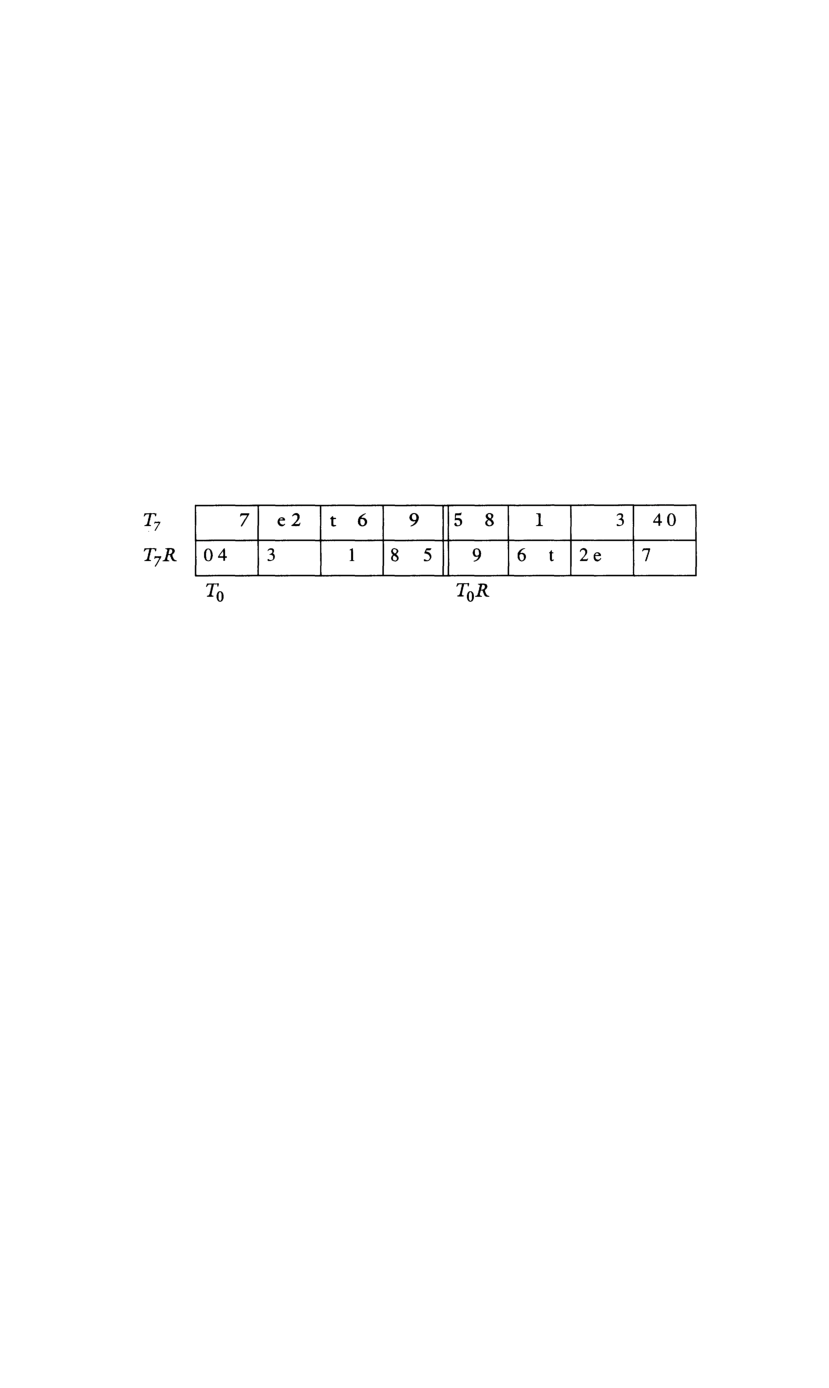
\includegraphics[width=5in]{figures/scotto-array.pdf}
		\caption[Self-derived row in Scotto's \emph{Tetralogy}]{Self-derived row in Scotto's \emph{Tetralogy}.}
    	\label{fig:scotto-array}
	\end{figure}
	
	\noindent Similarly to Ex.~\ref{self-folded}, the above matrix can be folded in order to obtain subsequent levels of derivation. Unlike Ex.~\ref{self-folded}, however, Scotto derives a rotated transform of $S$ from $\R\T_7(S)$. The rows in Fig.~\ref{fig:scotto-folded} are thus $\T_2(S), \R\T_2(S), \rho_6\R\T_2(S)$ and $\rho_6\T_2(S)$, where $\rho$ is the cyclical rotation operator.
	
	\begin{figure}[htbp]
    	\centering
		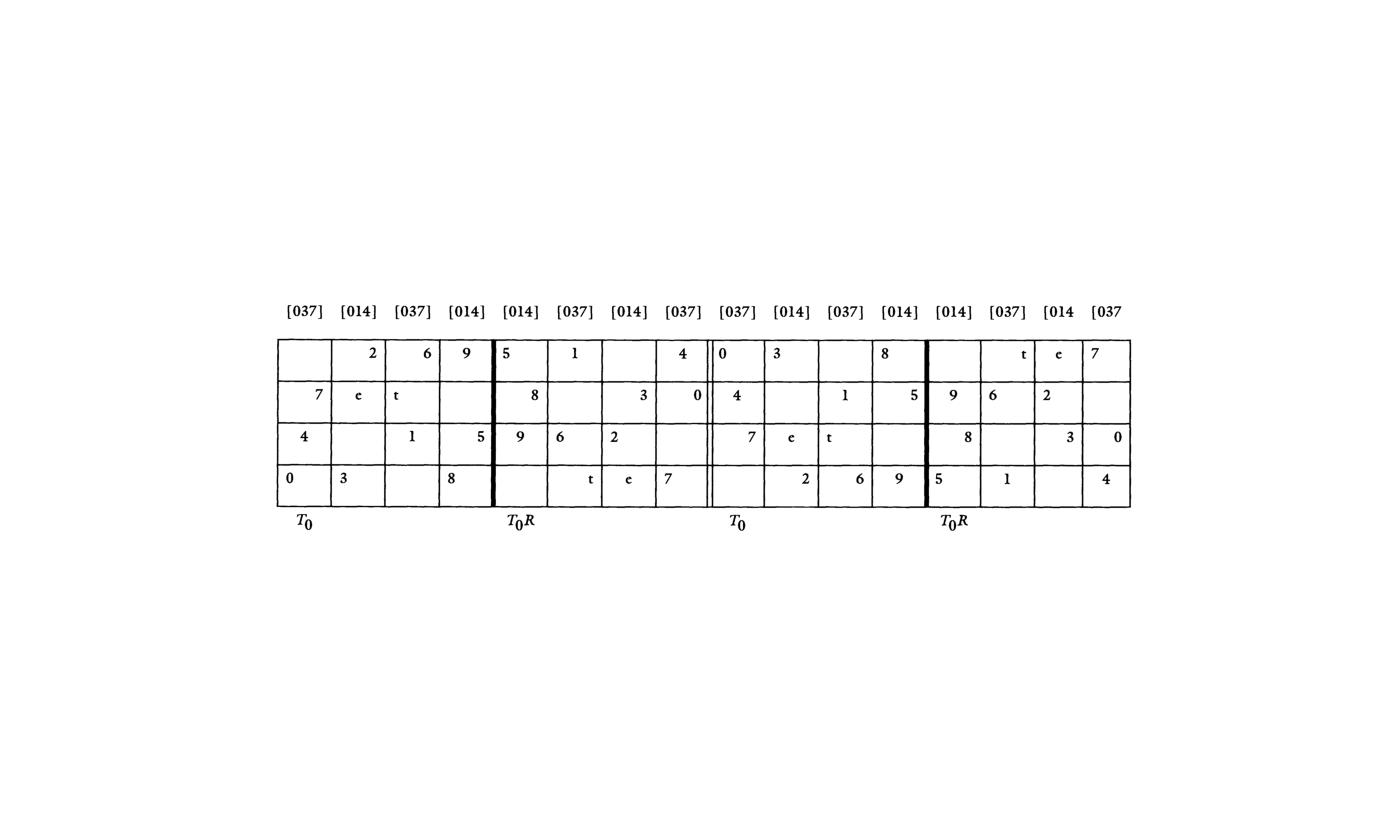
\includegraphics[width=6.5in]{figures/scotto-folded.pdf}
		\caption[Folded derivation in Scotto's \emph{Tetralogy}]{Folded derivation in Scotto's \emph{Tetralogy}.}
    	\label{fig:scotto-folded}
	\end{figure}
	
	\noindent In an entirely Schenkerian fashion, Scotto utilizes the folded array as the source material for the middle-ground structure of \emph{Tetralogy}. The only difference between the derivation array and the Schenkerian graph is that the $\T_2(S)$ now corresponds to the alto register, as seen in Fig.~\ref{fig:scotto-schenker1}. One of the foreground realizations of the Schenkerian graph in Fig.~\ref{fig:scotto-schenker1} is given in Fig.~\ref{fig:scotto-music1}. Rather than a strict serial composition, \emph{Tetralogy} employs a variety of prolongation procedures which are in line with its Schenkerian orientation, but unfortunately beyond the scope of this discussion.
	
	\begin{figure}[htbp]
    	\centering
		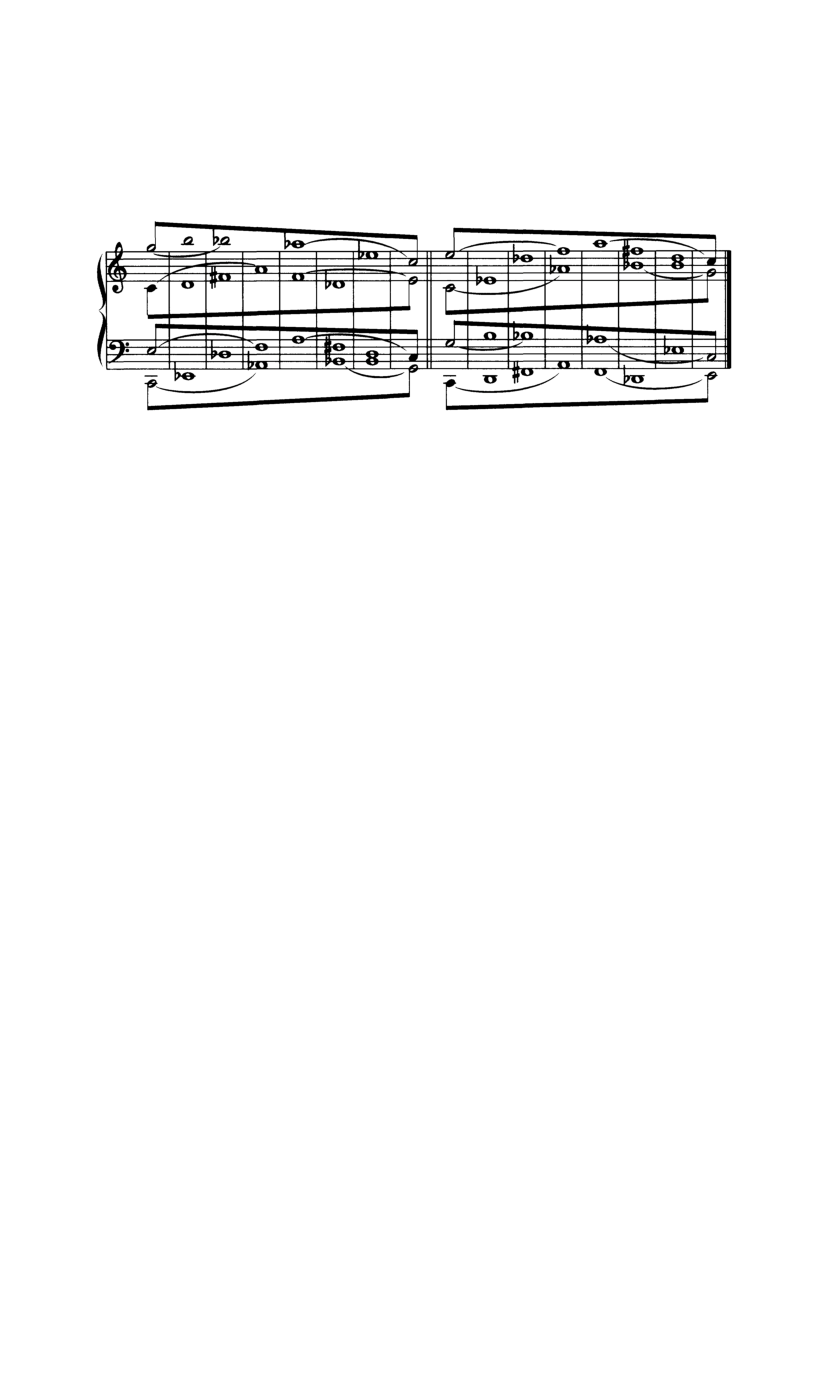
\includegraphics[width=6.5in]{figures/scotto-schenker1.pdf}
		\caption[Schenkerian middle-ground structure in Scotto's \emph{Tetralogy}]{Schenkerian middle-ground structure in Scotto's \emph{Tetralogy}.}
    	\label{fig:scotto-schenker1}
	\end{figure}
	
	\begin{figure}[htbp]
    	\centering
    	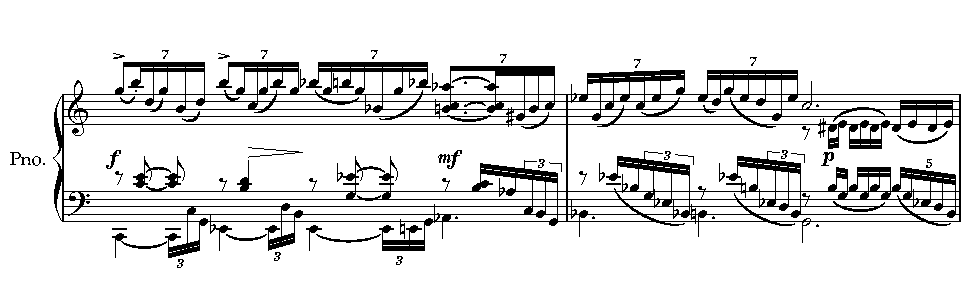
\includegraphics[width=6.5in]{figures/Scotto_1.pdf} %scotto-music1.pdf
		\caption[Musical realization of the middle-ground in Scotto's \emph{Tetralogy}]{Musical realization of the middle-ground in Scotto's \emph{Tetralogy}.}
    	\label{fig:scotto-music1}
	\end{figure}
	
	\noindent The idea of prolongation in \emph{Tetralogy} extends beyond the foreground musical surface, and is applied as well to the middle-ground structure itself, effectively pushing it further into the background of the piece. The prolongation of the first bar in Fig.~\ref{fig:scotto-schenker1} is depicted in Fig.~\ref{fig:scotto-schenker2}, and a musical realization thereof is displayed in Fig.~\ref{fig:scotto-music2}. 
	
	\begin{figure}[htbp]
    	\centering
    	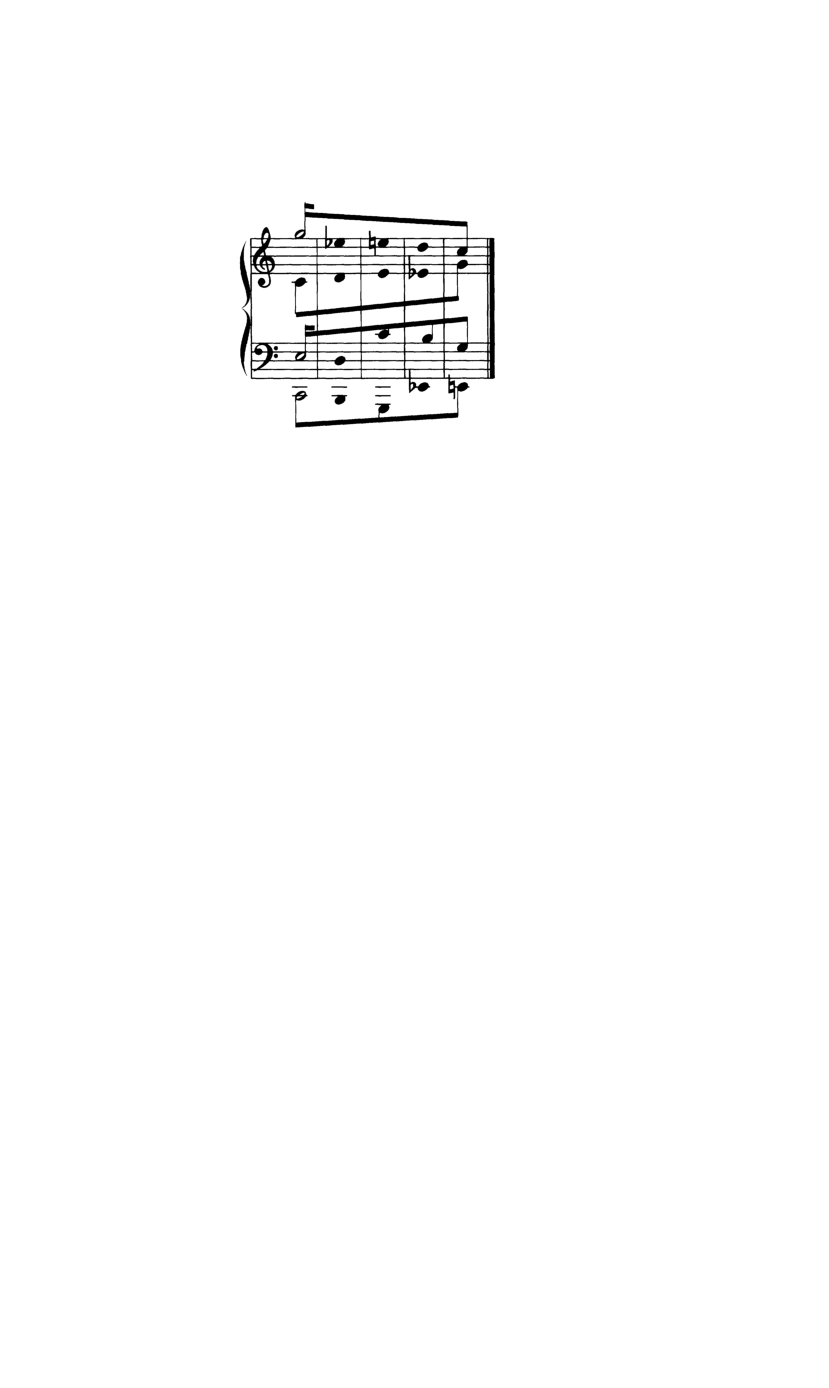
\includegraphics[width=2.2in]{figures/scotto-schenker2.pdf}
    	\caption[Prolongation of the middle-ground structure in Scotto's \emph{Tetralogy}]{Prolongation of the middle-ground structure in Scotto's \emph{Tetralogy}.}
    	\label{fig:scotto-schenker2}
	\end{figure}
	
	\begin{figure}[htbp]
    	\centering
    	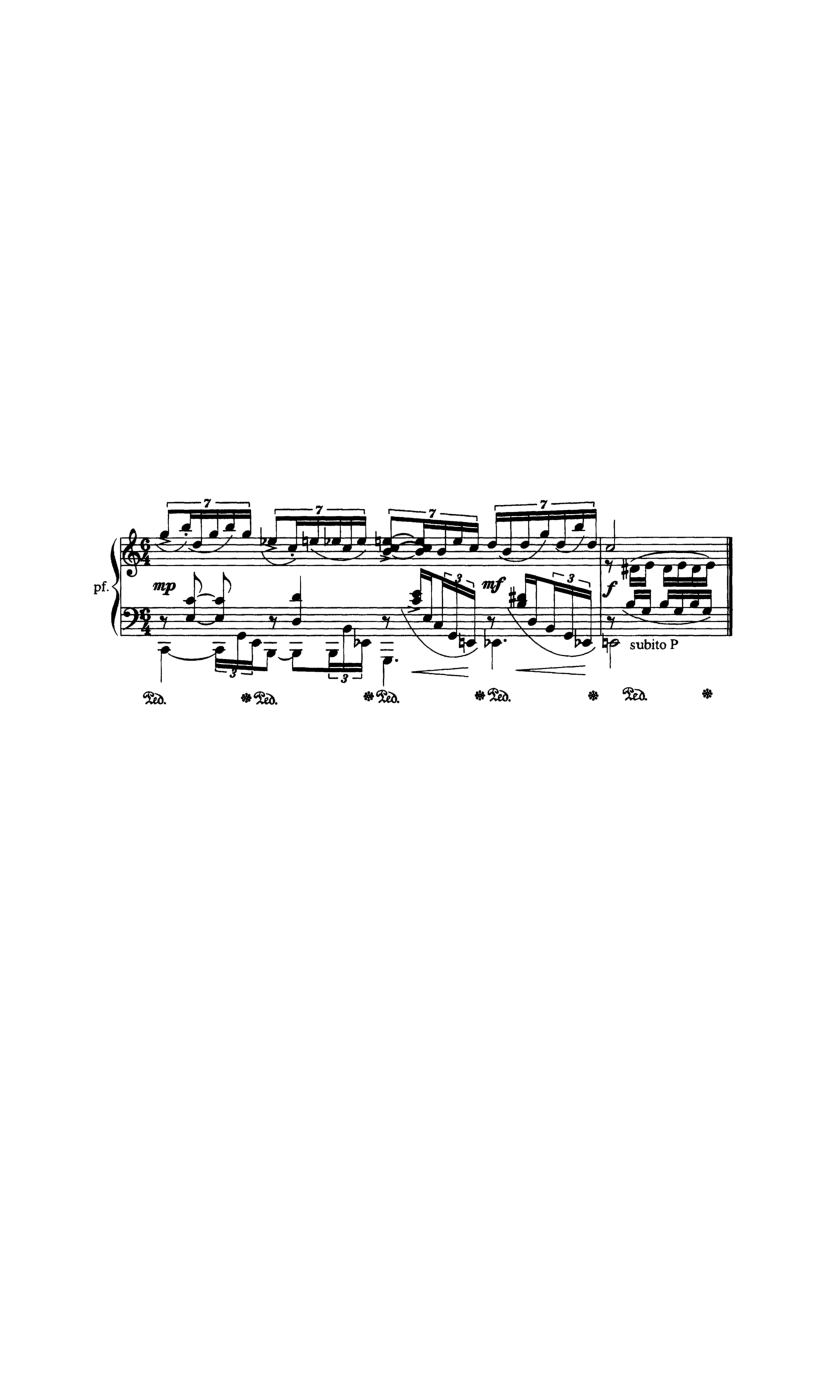
\includegraphics[width=6.5in]{figures/scotto-music2.pdf}
    	\caption[Musical realization of the prolonged middle-ground in Scotto's \emph{Tetralogy}]{Musical realization of the prolonged middle-ground in Scotto's \emph{Tetralogy}.}
    	\label{fig:scotto-music2}
	\end{figure}
\end{example}

\cite[217]{Starr1984} presents an algorithm for computing $2 \times 24$ combination matrices of self-derivation that consists of finding an segment at the beginning of an ordered set that can become an embedded segment in some transform of the set, then construct a combination matrix involving the retrograde by resolving any symmetries. There is no prior knowledge of the entire row, thus the row is actually composed by adding order constraints. Another procedure is introduced in \cite[222]{Starr1984} that utilizes Th.~\ref{starr-theorem} to construct self-derivation from general combinatoriality matrices by finding operations that resolve symmetries between the columns of the matrix. Although there is no requirement that the matrix be retrograde-invariant, the retrograde makes it arguably easier to work out the algorithm by hand. Ex.~\ref{ex:starr-algorithm-2} illustrates the latter procedure in which, similarly to the former, the entire row is discovered as a result of the procedure.

\begin{example}
	\label{ex:starr-algorithm-2}
    \cite[224]{Starr1984}
    Let $S = \{ 0, 1, 7, 2 \} | \{ 10, 9 \} | \{ 11, 4, 8, 5 \} | \{ 3, 6 \}$. Given that the complement of a row's first hexachord is always obtained from its second hexachord, a trivial case of hexachordal combinatoriality results when a row is matched with its retrograde. It is then possible to partition $S$ such that the combination matrix will have four columns:
    \begin{equation}
        A = \left[
        \begin{array}{c|c|c|c}
        	\{ 0, 1, 7, 2 \} & \{ 10, 9 \} & \{ 11, 4, 8, 5 \} & \{ 3, 6 \} \\
        	\{ 6, 3 \} & \{ 5, 8, 4, 11 \} & \{ 9, 10 \} & \{ 2, 7, 1, 0 \}
        \end{array}
        \right] \enspace.
    \end{equation}
    Now consider the cycles of $\T_{11}\I = (0 \; 11) (1 \; 10) (2 \; 9) (3 \; 8) (4 \; 7) (5 \; 6)$. In particular, the first column of $A$ will comprise the partial order $S_1 \cup \R(S_4)$, and this union will, in turn, map onto its hexachordal complement under $\T_{11}\I$, as it takes precisely one element from each of the operation's cycles, all of which have length two. Since the second column above is the complement of the first, it will also map onto its complement under $\T_{11}\I$. Because the third and fourth columns are mirrors of the first two, hexachordal combinatoriality under $\T_{11}\I$ is obtained in every column, that is, for the partial orders $S_1 \cup \R(S_4)$ and $S_2 \cup \R(S_3)$, as well as their retrogrades. The same result is not obtained between $S$ and $\T_{11}\I(S)$, that is, the first hexachord of $\T_{11}\I(S)$ is \emph{not} the complement of the first hexachord of $S$. This procedure yields the matrix $\hat{A}$.
    \begin{equation}
        \hat{A} = \left[
        \begin{array}{c|c|c|c}
        	\{ 0, 1, 7, 2 \} & \{ 10, 9 \} & \{ 11, 4, 8, 5 \} & \{ 3, 6 \} \\
        	\{ 6, 3 \} & \{ 5, 8, 4, 11 \} & \{ 9, 10 \} & \{ 2, 7, 1, 0 \} \\
        	\{ 11, 10, 4, 9 \} & \{ 1, 2 \} & \{ 0, 7, 3, 6 \} & \{ 8, 5 \} \\
        	\{ 5, 8 \} & \{ 6, 3, 7, 0 \} & \{ 2, 1 \} & \{ 9, 4, 10, 11 \}
        \end{array}
        \right] \enspace.
    \end{equation}
    The above can be construed as a sequence of four columnar realizations. It may be possible to derive members of the same row class from each column. If the total order class of the intersection of all columns is not empty, that is, if it contains the free aggregate and does not contain any symmetry, then Th.~\ref{starr-theorem} guarantees representatives of this row class can derived from each column. Let $C_1, C_2, C_3, C_4$ be the four columns of the matrix $\hat{A}$. It follows the row $V = \{ 11, 0, 1, 6, 10, 4, 7, 2, 9, 5, 3, 8 \}$ has the property that $T \in \Toc \{ \Ext[ C_1 \cup \R\T_1\I(C_2) \cup \T_1\I(C_3) \cup \R(C_4) ] \}$. Therefore $[V | \R\T_1\I(V) | \T_1\I(V) | \R(V)]$ can be derived from the columns of $\hat{A}$.
    \begin{equation*}
        \left[
        \begin{array}{cccccccccccc|cccccccccccc|c}
            & 0 & 1 &&&& 7 & 2 &&&& && 10 &&&&& 9 &&&&& & \\
            &&& 6 &&&&&&& 3 & & 5 && 8 & 4 & 11 &&&&&&& & \\
            \hline
            11 &&&& 10 & 4 &&& 9 &&& &&&&&&&&&&& 1 & 2 & \\
            &&&&&&&&& 5 && 8 &&&&&& 6 && 3 & 7 & 0 && & 2
        \end{array}
        \right. \cdots
    \end{equation*}
    \begin{equation}
        \cdots \left.
        \begin{array}{c|cccccccccccc|cccccccccccc}
            & &&&&&&& 11 & 4 & 8 && 5 && 3 &&&&&&& 6 &&& \\
            & &&&&& 9 &&&&& 10 & &&&&& 2 & 7 &&&& 1 & 0 & \\
            \hline
            & && 0 & 7 & 3 && 6 &&&&& & 8 && 5 &&&&&&&&& \\
            2 & 2 & 1 &&&&&&&&&& &&&& 9 &&& 4 & 10 &&&& 11
        \end{array} \right] \enspace.
    \end{equation}
\end{example}

Using columnar aggregates to compose combination matrices of self-derivation is further elaborated in \cite[226]{Starr1984} from the standpoint of explicitly building the columnar aggregates in the matrix from the cycles of some operation.

\begin{example}
    \cite[226, 227]{Starr1984}
    Let $S = \{ 0, 1, 7, 2 \} | \{ 10, 9, 11, 4 \} | \{ 8, 5, 3, 6 \} = S_1 | S_2 | S_3$ and consider the matrix $A = [S | \T_4(S) | \T_8(S)]^T$.
    \begin{equation}
        A = \left[
        \begin{array}{cccc|cccc|cccc}
        	0 & 1 & 7 & 2 & 10 & 9 & 11 & 4 & 8 & 5 & 3 & 6 \\
        	4 & 5 & 11 & 6 & 2 & 1 & 3 & 8 & 0 & 9 & 7 & 10 \\
        	8 & 9 & 3 & 10 & 6 & 5 & 7 & 0 & 4 & 1 & 11 & 2
        \end{array}
        \right] \enspace.
    \end{equation}
    Now let $V$ be in the total order class of the first columnar aggregate of $A$. Next, rewrite the first columnar aggregate of $A$ as the aggregate realization $A_1$.
    \begin{equation}
        A_1 = \begin{tikzcd}
            & 0 \arrow[dr] && 1 \arrow[dr] && 7 \arrow[dr] && 2 \arrow[dr] & \\
            * \arrow[r] \arrow[dr] \arrow[ur] & 4 \arrow[r] & * \arrow[r] \arrow[dr] \arrow[ur] & 5 \arrow[r] & * \arrow[r] \arrow[dr] \arrow[ur] & 11 \arrow[r] & * \arrow[r] \arrow[dr] \arrow[ur] & 6 \arrow[r] & * \\
            & 8 \arrow[ur] && 9 \arrow[ur] && 3 \arrow[ur] && 10 \arrow[ur] &
        \end{tikzcd}
    \end{equation}
    When the first column of $A$ is regarded as an aggregate realization, it becomes clearer that any $V \in \Toc(A_1)$ must be a succession of augmented triads, say, $V = \{ 4, 8, 0, 9, 1, 5, 11, 7, 3, 2, 10, 6 \}$. It is easy to see that linearizing $V$ from $A_1$ is possible, but it is not obvious whether some transform of $V$ can be linearized from the other columns of $A$. The answer depends on the chosen operation, $\T_4$ in this case, and on the chosen $S$. To verify that $A_2$ is a transform of $A_1$, it suffices to check whether there is a base-four $\R\T_n\M\I$ operation that maps $S_1 \pmod 4$ onto $S_2 \pmod 4$. This is easily verified, as indeed
    \begin{equation}
        S_1 \pmod 4 = \{ 0, 1, 3, 2 \} = \T_2\I(\{ 2, 1, 3, 0 \}) = \T_2\I \circ S_2 \pmod 4 \enspace.
    \end{equation}
    The above method works because the elements in each of $A_1$'s columns are incomparable, thus may be picked from each column in any order. In other words, $A_1$ could be flipped horizontally, say, and still have the same aggregate realization. Since all of $A$'s columns can be reduced $\mod 4$ by construction, it becomes enough to only consider each column's residue modulo four, and four-tone operations. Since $S_1 \pmod 4 = S_3 \pmod 4$, $V$ itself can be derived from $A_3$, and thus yielding the following derivation matrix, where the second column is $\T_2\I(V)$:
    \begin{multline}
        \left[
        \begin{array}{cccccccccccc|cccccc}
        	&& 0 && 1 &&& 7 && 2 && & 10 &&&&& 9 \\
        	4 &&&&& 5 & 11 &&&&& 6 & && 2 && 1 & \\
        	& 8 && 9 &&&&& 3 && 10 & & & 6 && 5 &&
        \end{array}
        \right. \cdots \\\\
        \cdots \left.
        \begin{array}{cccccc|cccccccccccc}
        	&& 11 && 4 & & & 8 &&&& 5 &&& 3 &&& 6 \\
        	3 &&&&& 8 & && 0 & 9 &&&& 7 &&& 10 & \\
        	& 7 && 0 && & 4 &&&& 1 && 11 &&& 2 &&
        \end{array}
        \right] \enspace.
    \end{multline}
    It may be possible to derive other rows from $A$ that are not based on the concatenation of cycles from an operation. Knowing that the columns of $A$ are related as aggregate realizations by the operation tuple $\mathcal{A} = [\T_0 \; \T_2\I \; \T_0]$, and regarding the $A_i$ as columnar aggregates, take $\hat{A} = \Ext[\bigcup_i(\mathcal{A}_i \circ A_i)]$. By Th.~\ref{starr-theorem}, any row that can be linearized from $\hat{A}$, will be in $\bigcap_i \Toc(A_i)$, and thus its $\mathcal{A}_i$-transform can be derive from each $i$-column of $A$. Below is the columnar aggregate $\hat{A}$.
    \begin{equation}
        \hat{A} = \begin{tikzcd}
            & 0 \arrow[r] \arrow[ddr] & 1 \arrow[r] \arrow[dr] & 7 \arrow[r] \arrow[ddr] & 2 \arrow[dr] & \\
            * \arrow[r] \arrow[dr] \arrow[ur] & 4 \arrow[r] \arrow[ur] & 5 \arrow[r] \arrow[dr] & 11 \arrow[r] \arrow[ur] & 6 \arrow[r] & * \\
            & 8 \arrow[r] \arrow[ur] & 9 \arrow[r] \arrow[uur] & 3 \arrow[r] \arrow[ur] & 10 \arrow[ur] &
        \end{tikzcd}
    \end{equation}
    It follows $\hat{V} = \{ 0, 1, 4, 8, 9, 5, 7, 2, 11, 3, 10, 6 \}$ can be linearized from $\hat{A}$, yielding the derivation matrix below:
    \begin{multline}
        \left[
        \begin{array}{cccccccccccc|cccccc}
        	0 &&&& 1 & 7 &&& 2 &&&&&&& 10 && \\
        	&&& 4 &&& 5 & 11 &&& 6 && 2 &&&& 1 & \\
        	& 8 & 9 &&&&&&& 3 && 10 && 6 & 5 &&& 7
        \end{array}
        \right. \cdots \\\\
        \cdots \left.
        \begin{array}{cccccc|cccccccccccc}
        	9 &&& 11 && 4 && 8 &&&&& 5 &&& 3 & 6 & \\
        	& 3 &&& 8 && 0 && 9 &&& 7 &&&&&& 10 \\
        	&& 0 &&&&&&& 4 & 1 &&& 11 & 2 &&&
        \end{array}
        \right] \enspace.
    \end{multline}
\end{example}

Ex.~\ref{ex:stingray} illustrates how self-derivation may be achieved in a $6 \times 144$ matrix by exploring the symmetries of an aggregate realization, and how such matrix may be used in an actual musical composition.

\begin{example}
    \label{ex:stingray}
    Consider the aggregate realization A.
    \begin{equation}
        A = \begin{tikzcd}
            & 0 \arrow[dddr] && 1 \arrow[dddr] & \\
            & 4 \arrow[ddr] && 5 \arrow[ddr] & \\
            & 8 \arrow[dr] && 9 \arrow[dr] & \\
            * \arrow[ur] \arrow[uur] \arrow[uuur] \arrow[dr] \arrow[ddr] \arrow[dddr] && * \arrow[ur] \arrow[uur] \arrow[uuur] \arrow[dr] \arrow[ddr] \arrow[dddr] && * \\
            & 11 \arrow[ur] && 10 \arrow[ur] & \\
            & 7 \arrow[uur] && 6 \arrow[uur] & \\
            & 3 \arrow[uuur] && 2 \arrow[uuur] &
        \end{tikzcd} \enspace.
    \end{equation}
    It is easily seen that $A$ is invariant under the set of operations $\Omega = \{ \T_0, \T_4, \T_8, \T_3\I, \T_7\I, \T_{11}\I \}$. Thus if $\rho \in \Toc(A)$, then also $\Omega_i(\rho) \in \Toc(A)$. It is also easy to see that $\R(\rho) \in \Toc(\R \circ \Omega_i(A))$. Now let $S = \{ 0, 1, 5, 8, 9, 4, 10, 3, 7, 6, 2, 11 \}$, and consider the combination matrix $\mathcal{A} = [\mathcal{A}_1 | \cdots | \mathcal{A}_6]$.
    \begin{equation}
        \mathcal{A} = \left[
        \begin{array}{cc|cc|cc|cc|cc|cc}
            0 & 1 & 5 & 8 & 9 & 4 & 10 & 3 & 7 & 6 & 2 & 11 \\
            4 & 5 & 9 & 0 & 1 & 8 & 2 & 7 & 11 & 10 & 6 & 3 \\
            8 & 9 & 1 & 4 & 5 & 0 & 6 & 11 & 3 & 2 & 10 & 7 \\
            11 & 10 & 6 & 3 & 2 & 7 & 1 & 8 & 4 & 5 & 9 & 0 \\
            7 & 6 & 2 & 11 & 10 & 3 & 9 & 4 & 0 & 1 & 5 & 8 \\
            3 & 2 & 10 & 7 & 6 & 11 & 5 & 0 & 8 & 9 & 1 & 4
        \end{array}
        \right] \enspace.
    \end{equation}
    By construction, every row of $\mathcal{A}$ is an $\Omega$-transform of $S$. Also by construction, every $\mathcal{A}_i$ is an instance of either $A$ or $\R(A)$, seen as a columnar aggregate, and thus $\Omega$-invariant. It follows a transform of $S$ can be derived from every $\mathcal{A}_i$. Since $\T_7(S) \in \Toc(\mathcal{A}_1)$ and $\R\T_0\I(S) \in \Toc(\mathcal{A}_2)$, self-derivation matrix $X$ is obtained.
    \begin{equation}
        X = \left[
        \begin{array}{cccccccccccc|cccccccccccc}
            &&&&& 11 && 10 &&&&&&& 6 &&&&& 3 &&&& \\
            &&&& 4 && 5 &&&&&&&&&& 9 &&&&&&& 0 \\
            &&& 3 &&&&& 2 &&&&& 10 &&&&&&&& 7 && \\
            && 0 &&&&&&& 1 &&&&&& 5 &&& 8 &&&&& \\
            & 8 &&&&&&&&& 9 && 1 &&&&&&&& 4 &&& \\
            7 &&&&&&&&&&& 6 &&&&&& 2 &&&&& 11 &
        \end{array}
        \right] \enspace.
    \end{equation}
    It is important to point out that, although the matrix $X$ could be extended to a $6 \times 144$ derivation matrix wherein all columns of $\mathcal{A}$ are presented, this could not be done using arbitrary transforms of $S$. Upon inspection, it follows that the transforms of $S$ that can be derived from $\mathcal{A}_1$ and $\mathcal{A}_5$ are in
    \begin{equation}
        \{ \T_3, \T_7, \T_{11}, \R\T_1, \R\T_5, \R\T_9, \T_0\I, \T_4\I, \T_8\I, \R\T_2\I, \R\T_6\I, \R\T_{10}\I \} \enspace.
    \end{equation}
    For the columns $\mathcal{A}_2, \mathcal{A}_3, \mathcal{A}_4$ and $\mathcal{A}_6$, the transforms of $S$ that can be derived are in
    \begin{equation}
        \{ \T_1, \T_5, \T_9, \R\T_3, \R\T_7, \R\T_{11}, \T_2\I, \T_6\I, \T_{10}\I, \R\T_0\I, \R\T_4\I, \R\T_8\I \} \enspace.
    \end{equation}
    Rather than a hinderance, this fact can be leveraged to explore contrasting harmonic regions. Fig.~\ref{fig:stingray} shows a musical realization of $X$:
    \begin{figure}[htbp]
        \centering
        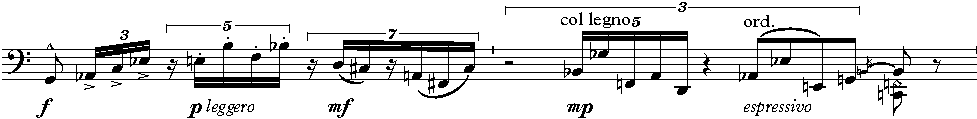
\includegraphics[width=6.5in]{figures/stingray-example.pdf}
        \caption[Self-derivation in Damiani's \emph{Stingray}.]{Self-derivation in Damiani's \emph{Stingray}.}
        \label{fig:stingray}
    \end{figure}
\end{example}

%--------------------------------------------------------------------------
\section{Final Remarks}

1. Goals

- The main motivation is to understand the construction of self-derivation precisely, that is, for any given row, whether it is capable of producing combination matrices of self-derivation.

- All the above shall be done in all generality, that is, for arbitrary $n$-tone temperament systems.

- Devise an algorithm to compute combination matrices of self derivation efficiently and to produce all possible representatives of matrices reduced to equivalence classes.

- Compare findings with \cite{Kowalski1987b}.

- The last chapter of the present work will deal with some musical applications of derivation techniques. Given the historical application of these techniques to almost exclusively the pitch domain, and in the interest of shedding new light onto such procedures, the compositional applications described will have a certain bias toward employing derivation in dimensions other than pitch.

1.1 Relevance

2. Limitations

- This paper will not deal with folded and skewed combination matrices, since those can be easily achieved from regular matrices.

- Although semi-magic squares have many interesting compositional applications, those will not be discussed. That includes the potatial for syntax that operating on semi-magic squares presents.

- Although most examples of derivation in the twentieth-century repertoire are of instrumental music, we shall not pursue the electroacoustic music avenue, nor algorithmic processes.

3. Tools and prior knowledge

- The theoretical framework will require previous knowledge of abstract and linear algebra, to the extend that many graduate texts in atonal music theory will require, and basic computer science. A working knowledge of twelve-tone theory is also required. Familiarity with such basic concepts as contour, pitch, and pitch-class spaces, intervals and interval classes, set classes, operations, and associated group-theoretic notions is assumed.

- As previously discussed, mathematics can greatly simplify our search for answers, and a solid mathematical theory of the musical objects that pertain to this study are a requirement for mature compositional decisions that involve the techniques here discussed. Anticipating, as much as possible, the symmetries of a musical construct of the sort with which we will be concerned can help a composer determine the outlook and feasibility of an entire piece. Mathematics is also crucial for constructing efficient computer algorithms that employ such techniques.
